\documentclass[12pt,a4paper]{article}

\usepackage[T1]{fontenc}
\usepackage[utf8]{inputenc}
\usepackage{lmodern}
\usepackage{microtype}
\usepackage[a4paper,margin=2.54cm]{geometry}
\usepackage{amsmath,amssymb}
\usepackage{graphicx}
\usepackage{array}
\usepackage{xcolor}
\usepackage{caption}
\usepackage{booktabs}
\usepackage{setspace}
\usepackage[mathlines]{lineno}
\usepackage[hidelinks]{hyperref}
\usepackage{subcaption}
\usepackage{tikz}
\usetikzlibrary{positioning,arrows.meta}

\captionsetup{
    font=small,
    labelfont=bf,
    labelsep=period
}
\captionsetup[table]{skip=10pt,position=top}

\setlength{\parindent}{1.5em}
\setlength{\parskip}{0pt}
\setlength{\emergencystretch}{2em}
% Line numbering is available for a later review version but is currently off.
% \modulolinenumbers[5]

\graphicspath{{./}{figures/}}
\newcolumntype{P}[1]{>{\raggedright\arraybackslash}p{#1}}

\usepackage[
backend=biber,
style=numeric,
sorting=none,
giveninits=true,
doi=true,
url=false,
isbn=false
]{biblatex}

\addbibresource{references_agglomerate_gnn.bib}

\begin{document}

\begin{center}
    {\Large\bfseries
    Graph-Based Compression of DEM-Resolved Agglomerate Morphology\par}
    \vspace{1.25em}
    {\normalsize Ali Khalifa and Heiko Briesen\par}
    \vspace{0.6em}
    {\small Chair of Process Systems Engineering, TUM School of Life Sciences,\par
    Technical University of Munich, Freising, Germany\par}
\end{center}

\vspace{1.25em}
\setstretch{1.5}

\begin{abstract}
	The internal morphology of particle agglomerates can affect oxygen access
	beyond conventional properties such as particle number, size and nominal
	fractal dimension. In this preliminary study, 135 synthetic monodisperse
	agglomerates were generated, relaxed by the discrete-element method and
	converted into particle-contact graphs. The supervised target was the mean
	geometric exposure: for each particle, uniformly distributed outward surface
	rays were tested for obstruction by all other particles, and the unobstructed
	fraction was averaged over the aggregate.

	A geometry-aware graph neural network (GNN) was evaluated using grouped
	five-fold cross-validation. Only the learned latent representation was supplied
	to the prediction head. The predefined compactness rule selected one latent
	variable, which predicted mean geometric exposure with RMSE $0.0160$, MAE
	$0.0128$ and $R^2=0.954$. The latent coordinate was most strongly associated
	with the requested fractal dimension and fractal prefactor
	($|\rho|=0.800$), and six conventional size and contact descriptors
	reconstructed it with grouped-CV $R^2=0.991$. Nevertheless, the GNN predicted
	exposure more accurately than particle count alone ($R^2=0.160$), the best
	individual classical descriptor model ($R^2=0.511$), and combined classical
	descriptor models (best $R^2=0.922$). The learned coordinate is therefore a
	compact task-specific representation of geometric exposure, although the
	target remains a line-of-sight proxy rather than a resolved oxygen-transport
	quantity.
\end{abstract}

\noindent\textbf{Keywords:} particle agglomerates; discrete-element method;
contact graphs; graph neural networks; latent morphology representation;
transport accessibility

% Activate for journal review only when required:
% \linenumbers

\section{Introduction}
\label{sec:introduction}

Transport models for biological and cohesive particle aggregates commonly
describe morphology using a small set of integral quantities, such as aggregate
diameter, porosity or fractal dimension. Such descriptors are useful, but they
do not uniquely determine the internal arrangement of the primary particles.
Aggregates with similar integral properties can still differ in connectivity,
surface exposure, shielding and the existence of internal transport pathways.
These structural differences may subsequently influence substrate or oxygen
accessibility and therefore the effective activity of an aggregate.

The broader research concept is to derive morphology-aware oxygen-transport
closures from particle-resolved CFD--DEM simulations and use them in
coarse-scale CFD--PBM or Euler--Lagrange reactor models. In that future
framework, a graph neural network would encode the detailed particle structure
into a compact morphology descriptor, while a reduced closure would combine
this descriptor with local reactor conditions to predict oxygen uptake, dynamic
response and the fraction of oxygen-limited cells.

Before conducting expensive coupled flow and transport simulations, the present
DEM-only study tests the feasibility of the structural part of this concept.
Its central hypothesis is that a particle-contact graph contains nonlocal
morphological information that can be compressed into a low-dimensional latent
representation without losing the information required to predict geometric
surface exposure. The study therefore addresses three preliminary questions:
\begin{enumerate}
    \item Can generated agglomerates be mechanically relaxed and converted
    consistently into particle-contact graphs?
    \item Can a GNN predict mean geometric exposure for parameter combinations
    withheld from training?
    \item How many latent variables are required to retain this structural
    information?
\end{enumerate}

The calculated target is intentionally limited to a geometric line-of-sight proxy.
This separation is important: the study validates the computational workflow
and the concept of morphology compression, while the physical relation to
oxygen transport remains a task for the proposed particle-resolved project.

The proof-of-concept study proceeds in six steps. First, synthetic
agglomerates are generated with different particle counts and physical sizes,
as well as with equal particle counts but different compactness settings and
random particle arrangements. Second, the artificial structures are relaxed
in a physical DEM environment to test whether they remain mechanically stable
under the selected particle and contact forces. Third, geometric exposure is
calculated from unobstructed outward surface rays. Fourth, each relaxed agglomerate is converted into a
particle-contact graph. Fifth, a GNN is trained to compress the graph into one
or more latent descriptors while retaining the information needed to predict
mean exposure. Finally, the learned descriptor is interpreted by comparing
it with conventional physical and graph-based measures, and its predictive
value is tested against particle count alone and against models using several
conventional descriptors together. The complete workflow is summarized in
Fig.~\ref{fig:study_workflow}.

\begin{figure}[!tbp]
	\centering
	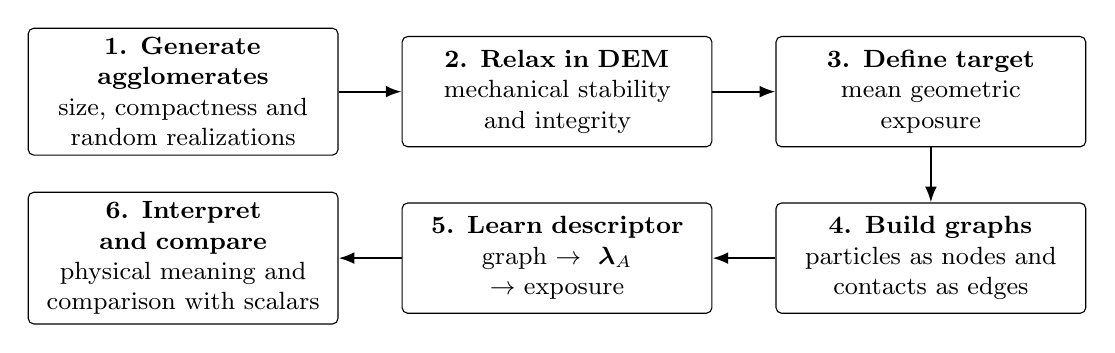
\begin{tikzpicture}[
		node distance=7mm and 8mm,
		workflowbox/.style={
			draw,
			rounded corners=2pt,
			align=center,
			minimum height=14mm,
			text width=3.7cm,
			font=\small
		},
		arrow/.style={-{Latex[length=2mm]}, thick}
	]
		\node[workflowbox] (generation) {
			\textbf{1. Generate agglomerates}\\
			size, compactness and\\random realizations
		};
		\node[workflowbox, right=of generation] (relaxation) {
			\textbf{2. Relax in DEM}\\
			mechanical stability\\and integrity
		};
		\node[workflowbox, right=of relaxation] (targets) {
			\textbf{3. Define target}\\
			mean geometric\\exposure
		};
		\node[workflowbox, below=of targets] (graphs) {
			\textbf{4. Build graphs}\\
			particles as nodes and\\contacts as edges
		};
		\node[workflowbox, left=of graphs] (compression) {
			\textbf{5. Learn descriptor}\\
			graph $\rightarrow \boldsymbol{\lambda}_A$\\$\rightarrow$ exposure
		};
		\node[workflowbox, left=of compression] (interpretation) {
			\textbf{6. Interpret and compare}\\
			physical meaning and\\comparison with scalars
		};

		\draw[arrow] (generation) -- (relaxation);
		\draw[arrow] (relaxation) -- (targets);
		\draw[arrow] (targets) -- (graphs);
		\draw[arrow] (graphs) -- (compression);
		\draw[arrow] (compression) -- (interpretation);
	\end{tikzpicture}
	\caption{Six-step workflow used to generate and relax synthetic
	agglomerates, represent them as graphs, learn a compact structural
	descriptor and evaluate its physical meaning and predictive value.}
	\label{fig:study_workflow}
\end{figure}

\section{Methodology and computational workflow}
\label{sec:preliminary_dem_gnn}

\subsection{Synthetic agglomerate ensemble}

The preliminary data set consists of monodisperse agglomerates generated with
the tunable particle--cluster and cluster--cluster aggregation formulation of
Filippov, Zurita and Rosner~\cite{Filippov2000}, following the efficient
hierarchical implementation described by Skorupski et
al.~\cite{Skorupski2014}. The method prescribes the mass--radius relation
\begin{equation}
    N=k_f\left(\frac{R_g}{r_p}\right)^{D_f},
    \label{eq:fractal_mass_radius}
\end{equation}
where $N$ is the number of primary particles, $r_p$ is their radius, $R_g$ is
the radius of gyration including the finite primary-particle radius, $D_f$ is
the requested fractal dimension and $k_f$ is the fractal prefactor.

Generation begins with stochastic 25-particle seed clusters. Starting from two
touching particles, further particles are placed at random orientations on the
radial shell required by Eq.~\eqref{eq:fractal_mass_radius}; placements are
accepted only when they establish contact without overlap. Equal-sized seed
clusters are subsequently combined hierarchically. Before each merge, both
subclusters are randomly rotated. Their prescribed center-of-mass separation
$R_{12}$ follows from the parallel-axis relation,
\begin{equation}
 R_{12}^{2}=
 r_p^2\frac{N^2}{N_1N_2}
 \left(\frac{N}{k_f}\right)^{2/D_f}
 -\frac{N}{N_2}R_{g,1}^{2}
 -\frac{N}{N_1}R_{g,2}^{2},
 \qquad N=N_1+N_2.
 \label{eq:cca_separation}
\end{equation}
A Monte Carlo orientation search identifies a non-overlapping configuration
whose first-contact separation agrees with $R_{12}$ within the prescribed
tolerance. The clusters are placed at this analytically determined
first-contact distance, guaranteeing connectivity without overlap while
allowing only a small, recorded deviation from the requested mass--radius law.
The particle counts $N=50$, 100 and 200 correspond to one, two and three
hierarchical merging levels, respectively, from the common 25-particle seeds.

Three morphology settings were used: $(D_f,k_f)=(1.8,1.3)$ for open,
$(2.2,1.1)$ for intermediate and $(2.6,0.8)$ for comparatively compact
agglomerates. The word ``compact'' is relative to the other fractal cases: the
cluster--cluster construction creates contact-connected fractal structures and
does not imply dense, nearly spherical packing. Dense spherical clusters would
require an additional restructuring or densification procedure
\cite{Ehrl2009}.

The data set comprises three primary-particle diameters, three particle counts,
three morphology settings and five independent random realizations per design
point,
\begin{equation*}
	3\ \text{diameters}\times3\ \text{particle counts}
	\times3\ \text{morphologies}\times5\ \text{realizations}
	=135\ \text{agglomerates}.
\end{equation*}
The details are summarized in Table~\ref{tab:sim_parameter}.


\begin{table}[!tbp]
	\centering
	\caption{Design variables used in the DEM investigation.}
	\label{tab:sim_parameter}
	\begin{tabular}{p{0.39\linewidth} p{0.51\linewidth}}
		\toprule
		\textbf{Design variable} & \textbf{Values} \\
		\midrule
		Primary-particle diameter $d_p$
		& $1.0$, $1.5$, $2.0\,\mu\mathrm{m}$ \\
		Number of particles $N$
		& $50$, $100$, $200$ \\
		Requested $(D_f,k_f)$ and morphology
		& $(1.8,1.3)$ open; $(2.2,1.1)$ intermediate;
		$(2.6,0.8)$ comparatively compact \\
		Random realizations
		& $5$ per parameter combination \\
		Total number of cases
		& $135$ \\
		\bottomrule
	\end{tabular}
\end{table}

Each realization was assigned a unique random seed. The generated particle
coordinates and radii were exported in formats suitable for DEM relaxation,
graph construction and visualization. All particles represented the same
material; no permanent bonds were prescribed, and the initial translational
and angular velocities were zero.

% Common crop for all three images:
% trim order: left, bottom, right, top

\begin{figure}[!tbp]
	\centering
	\begin{subfigure}[t]{0.32\textwidth}
		\centering
		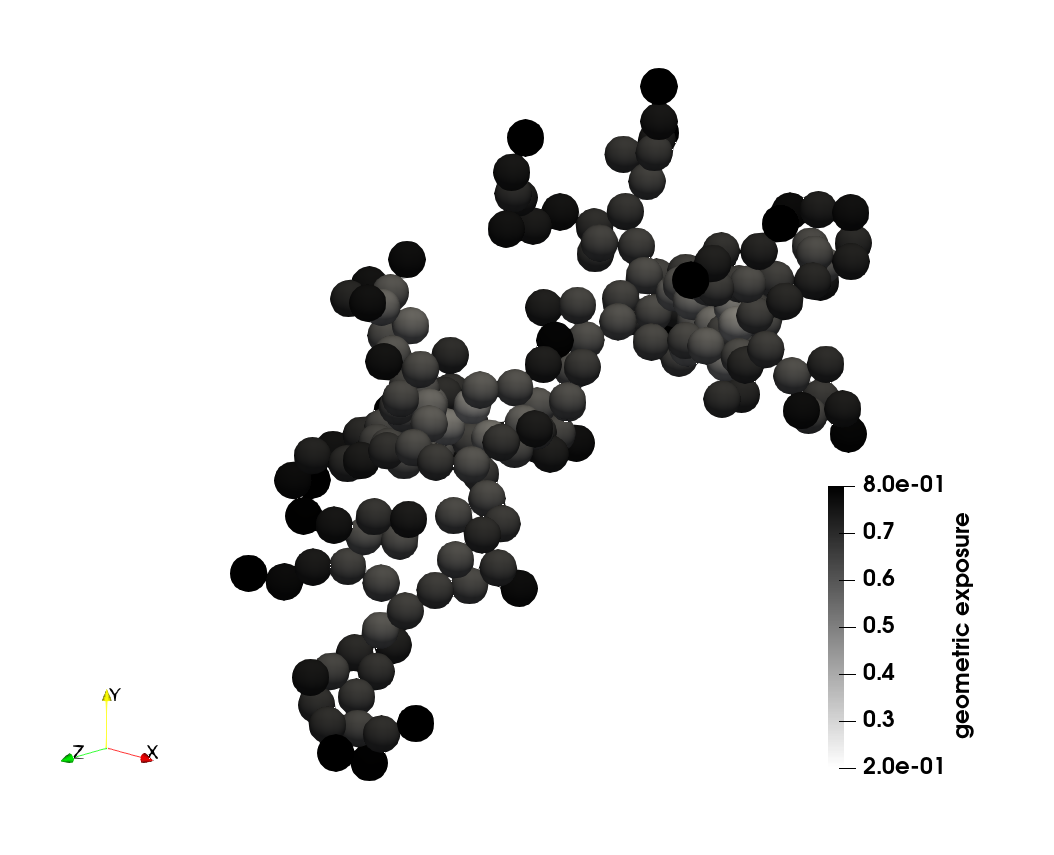
\includegraphics[
		width=1\linewidth,
	%	trim={450bp 5bp 450bp 5bp},
		clip
		]{./figures/open.png}
		\caption{Open aggregate}
		\label{fig:agg_open}
	\end{subfigure}
	\hfill
	\begin{subfigure}[t]{0.32\textwidth}
		\centering
		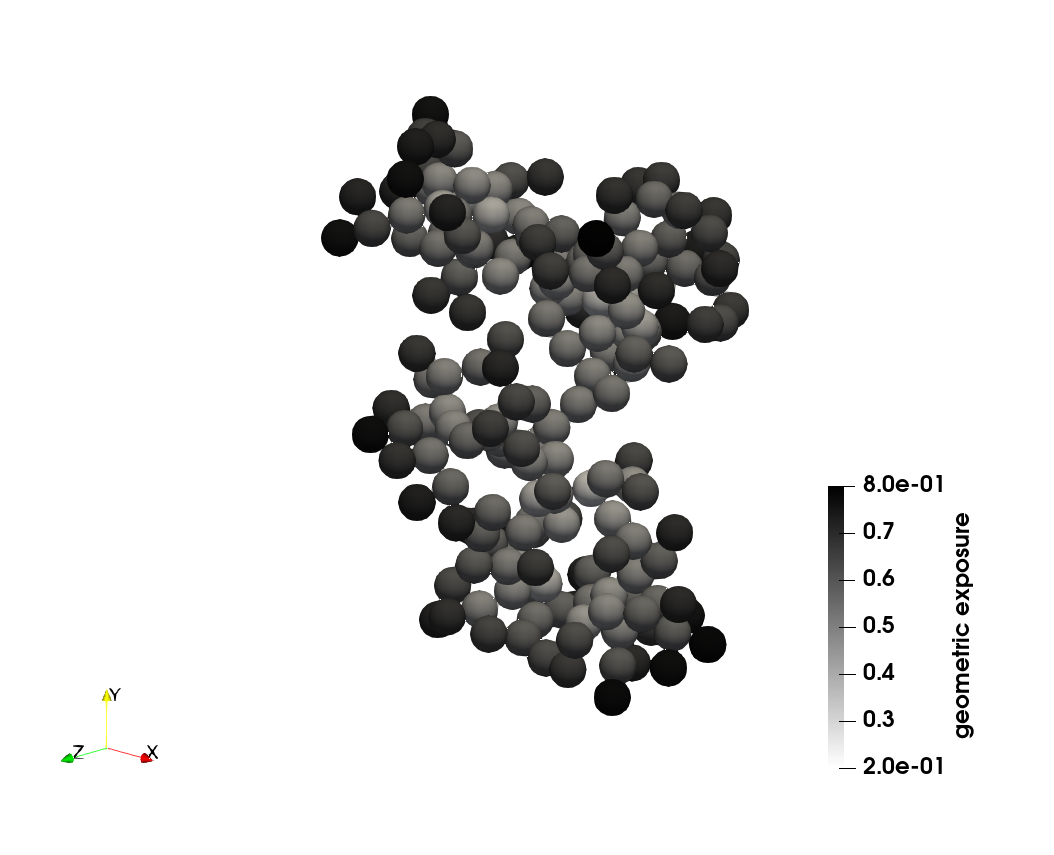
\includegraphics[
		width=1\linewidth,
	%	trim={450bp 5bp 450bp 5bp},
		clip
		]{./figures/intermediate.png}
		\caption{Intermediate aggregate}
		\label{fig:agg_intermediate}
	\end{subfigure}
	\hfill
	\begin{subfigure}[t]{0.32\textwidth}
		\centering
		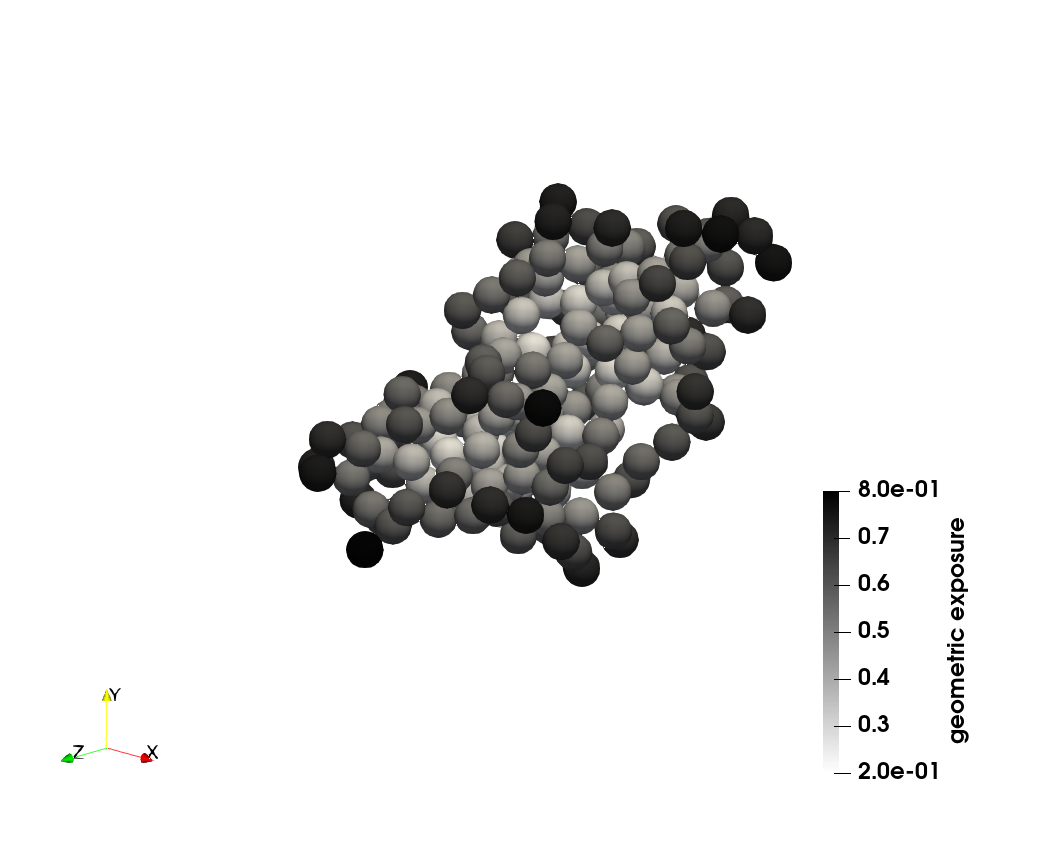
\includegraphics[
		width=1\linewidth,
	%	trim={450bp 5bp 450bp 5bp},
		clip
		]{./figures/compact.png}
		\caption{Comparatively compact aggregate}
		\label{fig:agg_compact}
	\end{subfigure}
	
	\caption{Representative post-DEM agglomerates illustrating the range of
		morphologies in the preliminary data set. The three agglomerates have the
		same primary-particle diameter ($d_p=$ 2 $\mu$m) and particle count ($N=$200) but different requested
		$(D_f,k_f)$ morphology settings. The particles are coloured according to
		their particle-level geometric exposure $a_i^{\mathrm{geo}}$, using a
		common colour scale from $0$ (all sampled outward directions blocked) to
		$1$ (all sampled outward directions unobstructed).}
	\label{fig:representative_agglomerates}
\end{figure}

\subsection{DEM relaxation and stability assessment}

The generated structures were mechanically relaxed using a soft-sphere DEM
formulation. Normal contact was described by Hertzian elastic repulsion and
regularized van der Waals attraction. The adhesive interaction is governed by
the Hamaker constant $A_H$ and a minimum surface separation $h_{\min}$, which
removes the singularity of the idealized interaction at vanishing separation
\cite{Hamaker1937,Israelachvili2011}. Tangential resistance was evaluated from
the contact history and limited by Coulomb friction. Rolling and torsional
resistance were also included. No permanent bonds were introduced; the relaxed
structures were maintained solely by adhesion and contact friction. The applied contact models are summarized in Table~\ref{tab:dem_contact_model}.
\begin{table}[!tbp]
	\centering
	\caption{Contact formulation used for DEM relaxation.}
	\label{tab:dem_contact_model}
	\begin{tabular}{P{0.32\linewidth} P{0.58\linewidth}}
		\toprule
		\textbf{Model component} &
		\textbf{Physical formulation} \\
		\midrule
		Normal interaction &
		Hertzian elastic repulsion combined with regularized van der Waals
		attraction \\
		
		Tangential interaction &
		History-dependent tangential force with Coulomb limitation \\
		
		Rolling resistance &
		Directional rolling-resistance torque \\
		
		Torsional resistance &
		Resistance to relative twisting at a contact \\
		
		Near-contact regularization &
		Limitation of nonphysical normal-force states near contact \\
		
		Permanent bonds &
		None \\
		\bottomrule
	\end{tabular}
\end{table}

Although the numerical setup permits multiple material types, identical
properties were used for every interaction in the present monodisperse study.
\begin{table}[!tbp]
	\centering
	\caption{Particle and contact parameters used in the DEM relaxation.
		The primary-particle diameter was varied, while the remaining properties
		were held constant.}
	\label{tab:dem_material_parameters}
	\begin{tabular}{p{0.39\linewidth} p{0.16\linewidth} p{0.29\linewidth}}
		\toprule
		\textbf{Property} & \textbf{Symbol} & \textbf{Value} \\
		\midrule
		Particle shape
		& -- & Sphere \\
		Primary-particle diameter
		& $d_p$ & $1.0$, $1.5$, $2.0\,\mu\mathrm{m}$ \\
		Reference particle density
		& $\rho_p$ & $1050\,\mathrm{kg\,m^{-3}}$ \\
		Young's modulus
		& $E$ & $1.0\times10^{9}\,\mathrm{Pa}$ \\
		Poisson ratio
		& $\nu$ & $0.45$ \\
		Coefficient of restitution
		& $e$ & $0.20$ \\
		Sliding-friction coefficient
		& $\mu$ & $0.30$ \\
		Rolling-friction coefficient
		& $\mu_r$ & $0.01$ \\
		Hamaker constant
		& $A_H$ & $3.028\times10^{-20}\,\mathrm{J}$ \\
		Minimum separation distance
		& $h_{\min}$ & $4.0\times10^{-10}\,\mathrm{m}$ \\
		\bottomrule
	\end{tabular}
\end{table}

The primary-particle diameters of $1.0$--$2.0\,\mu\mathrm{m}$ represent the
characteristic micrometre scale of many bacterial cells
\cite{LevinAngert2015}. The range is intentionally narrow:
its purpose in this preliminary study is to test whether the graph workflow
remains consistent when the physical length scale changes, while particle
number and morphology are varied independently. The density
$\rho_p=1050\,\mathrm{kg\,m^{-3}}$ represents a water-rich particle only
slightly denser than the surrounding liquid. Measurements for
\textit{Escherichia coli}, for example, place the buoyant density near
$1080$--$1105\,\mathrm{kg\,m^{-3}}$ \cite{MartinezSalas1981,Woldringh1981}.
The slightly lower reference value used here is therefore an idealized
near-neutral-buoyancy choice rather than a species-specific measurement. The
Poisson ratio $\nu=0.45$ represents a nearly incompressible effective particle.

The remaining mechanical parameters define a controlled relaxation model and
must not be interpreted as a calibrated constitutive description of a
particular microorganism. Reported effective bacterial-envelope moduli are
commonly in the MPa range and depend strongly on species, physiological state
and measurement protocol \cite{Deng2011,Lee2024}; the present value
$E=1\,\mathrm{GPa}$ was selected as a stiff numerical contact parameter to
restrict overlap during relaxation. The low restitution coefficient provides
strong damping, whereas the sliding- and rolling-friction coefficients resist
relative translation and rotation. The adopted Hamaker constant is of the
conventional $10^{-20}\,\mathrm{J}$ order associated with dispersion
interactions, but its effective value depends on the interacting materials and
the intervening liquid \cite{Israelachvili2011}. Accordingly, elasticity,
dissipation, friction and adhesion should be varied in a sensitivity study and
calibrated before applying the model to a specific bioaggregate. The relevant particle and contact parameters used in the present DEM relaxation simulations are listed in Table~\ref{tab:dem_material_parameters}.

%The particle density is inherited from the particle initialization data. Its
%value should therefore be verified directly in these files before the present
%study is submitted for publication.
%
%For the specified Hamaker constant and minimum separation, the corresponding
%planar work-of-adhesion estimate is
%\begin{equation}
% W=\frac{A_H}{12\pi h_{\min}^{2}}
%   \approx 5.0\times10^{-3}\,\mathrm{J\,m^{-2}}.
%\end{equation}
%This value characterizes the effective adhesion used in the preliminary
%relaxation and is not presented as a universally valid biological material
%constant.
The relaxation simulations were performed with a physical time step of
$\Delta t=5.0\times10^{-11}\,\mathrm{s}$ and were run for up to $300000$ time
steps, corresponding to a maximum physical duration of
$1.5\times10^{-5}\,\mathrm{s}=15\,\mu\mathrm{s}$. The purpose of this DEM stage
was to obtain mechanically stable structures and to verify that the
artificially generated agglomerates remained intact under the selected
elasticity, dissipation, friction and adhesive-contact conditions without
permanent bonds. The suitability of the time step was checked every $1000$
steps against the characteristic contact and neighbour-list time scales.
Particle and pair-interaction data were written every $20000$ steps,
corresponding to output intervals of $1\,\mu\mathrm{s}$. Gravity was not
activated because the simulation focused on internal contact-scale relaxation
without sedimentation or an externally imposed loading direction.

The particle output contained positions, radii, particle IDs and velocities,
whereas the pair output contained interacting particle IDs, gap, overlap,
contact area, normal and tangential forces, total force and torque. These data
were converted to VTK for inspection and subsequent graph construction.
Because the adhesive interaction also acts across a finite gap, a reported
particle pair does not necessarily represent a geometrically touching contact.
The pairs were therefore classified using
\begin{equation}
	\delta_{ij}
	=r_i+r_j-\lVert\boldsymbol{x}_i-\boldsymbol{x}_j\rVert .
\end{equation}
Pairs satisfying
$\delta_{ij}/d_{\mathrm{ref}}\geq-10^{-6}$ were treated as touching. This small
tolerance retains numerically near-touching pairs while excluding separated
neighbours interacting only through finite-range adhesive forces.

For each case, particle and contact VTK files were matched by time step. An
agglomerate was considered relaxed when, over three consecutive output
intervals,
\begin{equation}
	\frac{\Delta x_{\mathrm{RMS}}}{d_p}\leq10^{-4},
	\qquad
	1-\frac{|C_k\cap C_{k+1}|}{|C_k\cup C_{k+1}|}\leq0.01,
\end{equation}
where $C_k$ denotes the set of particle contacts at time step $k$. These
criteria require both the particle positions and the contact network to become
nearly stationary.

Agglomerate integrity was evaluated independently using connected-component
analysis. Each particle was treated as a graph node and every reported
particle-pair interaction as an undirected edge. All 135 final structures
contained exactly one connected component with a largest-component fraction of
unity. Thus, none of the artificially generated agglomerates fragmented during
the DEM relaxation.

\subsection{Effective fractal-dimension characterization}
\label{sec:measured_fractal_dimension}

The fractal dimensions specified during agglomerate generation define the
requested morphology settings. Since the generated structures contain only
\(50\)--\(200\) primary particles and are subsequently relaxed by DEM, these
input values should not be interpreted as exact measured properties of every
final structure. The relaxed agglomerates were therefore characterized using
two complementary finite-scale methods. Both methods are commonly used to
characterize particle aggregates, although their estimates can depend on the
available scale range and the finite number of primary particles
\cite{Bushell2002,Theiler1990}.

The first estimate was based on the mass--radius scaling relation commonly
used for fractal particle aggregates \cite{Sorensen2001,Bushell2002},
\begin{equation}
	N(r)\propto r^{D_f},
\end{equation}
where \(N(r)\) is the number of particle centres within a distance \(r\) from
the agglomerate centre of mass. After calculating the distance of every
particle centre from the agglomerate centre of mass, the particles were sorted
according to this radial distance. The effective fractal dimension was then
obtained from the slope of
\begin{equation}
	\log N(r)=D_f\log r+C.
\end{equation}
Only the range containing \(10\)--\(80\,\%\) of the particles was included in
the regression. The innermost region was excluded because it contains only a
small number of particles, while the outermost region is strongly affected by
the finite boundary of the agglomerate.

A second estimate was obtained using the box-counting method
\cite{Liebovitch1989,ForoutanPour1999,Theiler1990}. The particle centres were
covered by a three-dimensional Cartesian grid with box size \(\epsilon\), and
the number of boxes containing at least one particle centre,
\(N_{\mathrm{box}}(\epsilon)\), was counted. The effective box-counting
dimension follows from
\begin{equation}
	N_{\mathrm{box}}(\epsilon)
	\propto \epsilon^{-D_f},
\end{equation}
and was calculated as the slope of
\(\log N_{\mathrm{box}}\) against \(\log(1/\epsilon)\).

Before box counting, each agglomerate was translated to its centre and aligned
with its principal axes. Twelve logarithmically spaced box sizes were
evaluated. For each box size, 32 shifted grids were tested and the smallest
occupied-box count was retained to reduce sensitivity to the arbitrary grid
origin. Scales for which nearly all particles occupied separate boxes, as well
as scales for which the complete agglomerate occupied approximately one box,
were excluded. Such scale selection is important because both limits contain
little information about the intermediate spatial scaling
\cite{ForoutanPour1999,Theiler1990}.

\subsection{Graph representation and geometric-exposure target}

Each selected agglomerate snapshot was represented as a contact graph. Primary particles
form the nodes, while only geometrically touching or numerically near-touching
pairs satisfying $\delta_{ij}/d_{\mathrm{ref}}\geq-10^{-6}$ form the edges.
Separated attractive neighbours were excluded. This choice gives the graph a
clear geometrical interpretation and prevents its topology from depending on
the finite interaction cutoff of the adhesive model. Every retained pair was
stored in both directions for message passing. Thus, an agglomerate with $N$
particles and $N_c$ retained contacts has $N$ nodes and $2N_c$ directed edges.
All 135 agglomerates yielded valid graphs and were included in the analysis;
no case was skipped.

Three node features were available after preprocessing. The minimal model used
the two nonconstant structural scalars
\begin{equation}
 \boldsymbol{x}_i=
 \left[
   \frac{|\boldsymbol{x}_i-\boldsymbol{x}_c|}{R_g},\;
   z_i
 \right],
\end{equation}
where $d_{\mathrm{ref}}$ is twice the median particle radius,
$\boldsymbol{x}_c$ is the agglomerate center, $R_g$ is the radius of gyration,
and $z_i$ is the coordination number. The third available node feature,
$r_i/d_{\mathrm{ref}}$, is approximately $0.5$ for all present monodisperse
particles and was therefore omitted from the minimal model.

The processed DEM data contained 22 available contact features, including
normalized distance and overlap, gap, contact area, force and torque quantities
and contact-state flags. For the minimal model, only the normalized centre
distance $d_{ij}/d_{\mathrm{ref}}$ was selected from these stored contact
features, because connectivity and interparticle geometry are the quantities
directly relevant to the geometric-exposure target considered here. The graph
connectivity and normalized relative-position vector were additionally used
for message passing. The remaining available contact features were retained
for possible sensitivity studies but were not supplied to the reported model.

Geometric exposure was calculated independently of the convex hull. For each
particle $i$, $M=512$ approximately uniform unit directions
$\boldsymbol{s}_m$ were generated on the sphere using a deterministic Fibonacci
construction. A ray was started immediately outside the particle surface at
$\boldsymbol{x}_i+(r_i+\varepsilon)\boldsymbol{s}_m$ and propagated along the
outward normal $\boldsymbol{s}_m$. As illustrated in
Fig.~\ref{fig:ray_tracing_exposure}, a direction was classified as blocked if
the corresponding ray intersected any other particle; otherwise, it was
classified as unobstructed. Let $b_{im}=1$ for a blocked ray and $b_{im}=0$ for
an unobstructed ray. The particle-level exposure and the aggregate target are
\begin{align}
	a_i^{\mathrm{geo}} &= \frac{1}{M}\sum_{m=1}^{M}(1-b_{im}),\\
	\overline{a}_{\mathrm{geo}} &=
	\frac{1}{N}\sum_{i=1}^{N}a_i^{\mathrm{geo}}.
\end{align}

\begin{figure}[!tbp]
	\centering
	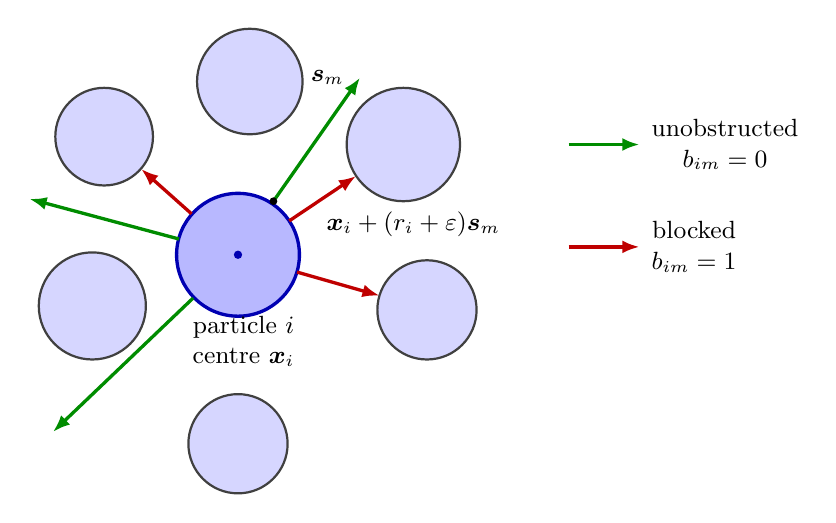
\begin{tikzpicture}[
		x=1cm,y=1cm,
		particle/.style={draw=black!75,thick,fill=blue!16},
		tested/.style={draw=blue!70!black,very thick,fill=blue!28},
		clear ray/.style={-{Latex[length=2.2mm]},very thick,green!55!black},
		blocked ray/.style={-{Latex[length=2.2mm]},very thick,red!75!black},
		label text/.style={font=\small,align=center}
	]
		% Neighbouring particles are drawn first so that the rays remain visible.
		\foreach \x/\y/\r in {
			4.55/0.55/0.63,
			4.25/2.65/0.72,
			2.30/3.45/0.67,
			0.45/2.75/0.62,
			0.30/0.60/0.68,
			2.15/-1.15/0.63}
			\draw[particle] (\x,\y) circle (\r);

		% Particle whose exposure is evaluated.
		\coordinate (C) at (2.15,1.25);
		\draw[tested] (C) circle (0.78);
		\fill[blue!70!black] (C) circle (1.5pt);
		\node[label text,below right=6.5mm and -7mm of C]
			{particle $i$\\centre $\boldsymbol{x}_i$};

		% Unobstructed rays extend into the surroundings.
		\draw[clear ray] (2.6,1.93) -- (3.70,3.50);
		\draw[clear ray] (1.40,1.45) -- (-0.50,1.96);
		\draw[clear ray] (1.58,0.70) -- (-0.20,-1.00);

		% Blocked rays stop at the first neighbouring particle.
		\draw[blocked ray] (2.90,1.03) -- (3.95,0.73);
		\draw[blocked ray] (2.80,1.68) -- (3.65,2.25);
		\draw[blocked ray] (1.56,1.77) -- (0.92,2.34);

		% Ray-start offset and direction annotation.
		\fill[black] (2.6,1.93) circle (1.4pt);
		\node[label text,above right=1mm and 10mm of C,shift={(0,0)}]
			{$\boldsymbol{x}_i+(r_i+\varepsilon)\boldsymbol{s}_m$};
		\node[label text,right] at (2.95,3.5) {$\boldsymbol{s}_m$};

		% Compact legend.
		\draw[clear ray] (6.35,2.65) -- (7.25,2.65);
		\node[label text,right] at (7.28,2.65)
			{unobstructed\\$b_{im}=0$};
		\draw[blocked ray] (6.35,1.35) -- (7.25,1.35);
		\node[label text,right] at (7.28,1.35)
			{blocked\\$b_{im}=1$};
	\end{tikzpicture}
	\caption{Schematic of the ray-tracing calculation for one particle $i$.
		Rays start just outside its surface and follow sampled outward directions
		$\boldsymbol{s}_m$. A ray is blocked when it intersects another particle;
		otherwise, it contributes to the exposed fraction. For clarity, only a
		two-dimensional section and a small subset of rays are shown; the actual
		calculation distributes $M=512$ directions over the complete sphere.}
	\label{fig:ray_tracing_exposure}
\end{figure}

Thus, $a_i^{\mathrm{geo}}=1$ means that all sampled outward directions are
unobstructed, whereas $a_i^{\mathrm{geo}}=0$ means that every sampled direction
is blocked. The reported calculation used zero probe-radius inflation, so rays
were blocked by the physical particle radii. Unlike the former contact-depth
proxy, this definition can assign low or high exposure to particles that are
close to the aggregate boundary but are not convex-hull vertices. It also
accounts directly for shadowing by particles located farther along a surface
direction. Nevertheless, $\overline{a}_{\mathrm{geo}}$ remains a purely
geometrical line-of-sight measure; it does not include pore diffusion, flow,
reaction or oxygen uptake.

\subsection{GNN compression and training}

In addition to the stored node and edge features, the model uses the particle
coordinates relative to the aggregate centre and normalized by the reference
diameter $d_{\mathrm{ref}}$. The corresponding relative-position vector is
assigned to every directed edge. Random rigid rotations are applied during
training to prevent the model from associating the target quantity with a
particular aggregate orientation.

The node and edge inputs are embedded into a hidden space of dimension 64.
Six residual GINE message-passing layers with layer normalization and dropout
are then applied. The message-passing depth allows information to propagate
over extended paths through the aggregate, while the residual connections
reduce optimization difficulties and the loss of local information. Graph-level
mean, maximum and size-sensitive normalized-sum pooling are combined to form a
graph-derived aggregate representation. This representation alone is
compressed through the latent bottleneck into a morphology vector
\begin{equation}
	\boldsymbol{\lambda}_A =
	\left[\lambda_1,\ldots,\lambda_{n_\lambda}\right]
	\in \mathbb{R}^{n_\lambda},
\end{equation}
where the latent dimension $n_\lambda$ is treated as a model hyperparameter.
Candidate values $n_\lambda\in\{1,2,3,4\}$ are evaluated by grouped
cross-validation. Thus, the GNN learns the values of the latent components,
whereas their required number is determined from the predictive performance
and model-complexity comparison.

No separately calculated aggregate-level descriptors are supplied to either
the latent bottleneck or the prediction head. Aggregate size, spatial extent
and connectivity can nevertheless be inferred from the number and arrangement
of nodes, their normalized coordinates, the contact topology and the
size-sensitive normalized-sum pooling term. A two-layer prediction head maps
only $\boldsymbol{\lambda}_A$ to the supervised exposure target,
\begin{equation}
	\widehat{y}_A=\widehat{\overline{a}}_{\mathrm{geo}}.
\end{equation}

Training used Adam with a learning rate of $10^{-3}$, weight decay of $10^{-5}$,
batch size 16 and random seed 7. The targets were standardized using only the
respective training data. A validation subset and early stopping were used to
retain the best model in each fold instead of automatically selecting the last
training epoch.


% In the document
\begin{figure}[!tbp]
	\centering
	\resizebox{0.99\textwidth}{!}{%
	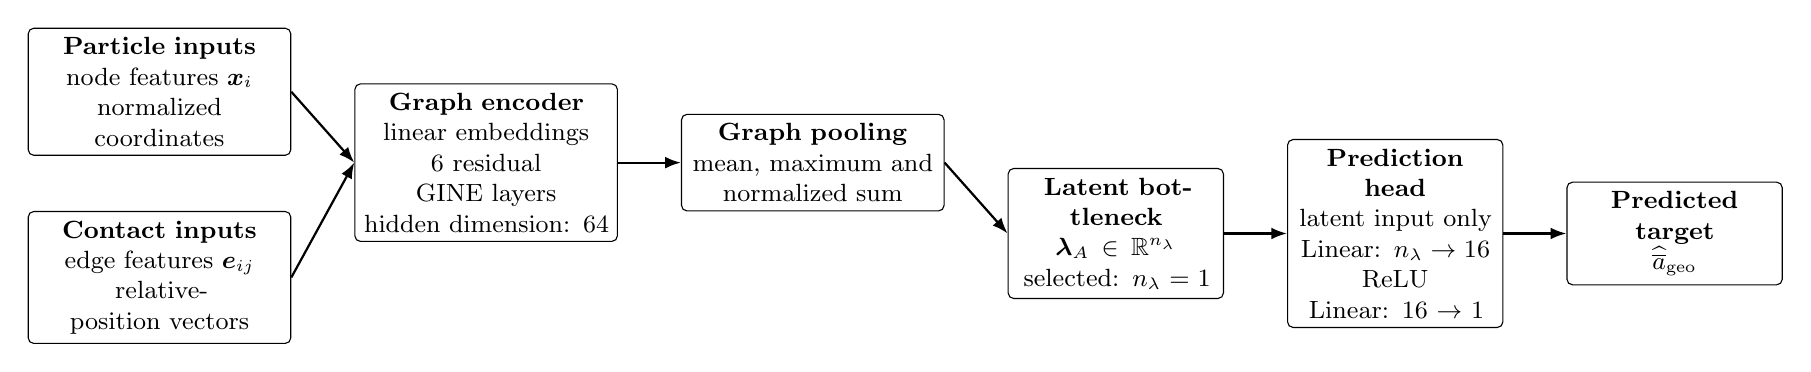
\begin{tikzpicture}[
		node distance=7mm and 8mm,
		block/.style={
			draw,
			rounded corners=2pt,
			align=center,
			minimum height=11mm,
			text width=3.1cm,
			font=\small
		},
		smallblock/.style={
			draw,
			rounded corners=2pt,
			align=center,
			minimum height=10mm,
			text width=2.5cm,
			font=\small
		},
		arrow/.style={-{Latex[length=2mm]}, thick}
		]
		
		% Graph-level inputs
		\node[block] (nodeinput) {
			\textbf{Particle inputs}\\
			node features $\boldsymbol{x}_i$\\
			normalized coordinates
		};
		
		\node[block, below=of nodeinput] (edgeinput) {
			\textbf{Contact inputs}\\
			edge features $\boldsymbol{e}_{ij}$\\
			relative-position vectors
		};
		
		% GNN
		\node[block, right=of nodeinput, yshift=-9mm] (gine) {
			\textbf{Graph encoder}\\
			linear embeddings\\
			$6$ residual GINE layers\\
			hidden dimension: $64$
		};
		
		% Pooling
		\node[block, right=of gine] (pooling) {
			\textbf{Graph pooling}\\
			mean, maximum and\\
			normalized sum
		};
		
		% Latent representation
		\node[smallblock, right=of pooling, yshift=-9mm] (latent) {
			\textbf{Latent bottleneck}\\
			$\boldsymbol{\lambda}_A
			\in\mathbb{R}^{n_\lambda}$\\
			selected: $n_\lambda=1$
		};
		
		% Prediction head
		\node[smallblock, right=of latent] (head) {
			\textbf{Prediction head}\\
			latent input only\\
			Linear: $n_\lambda\rightarrow16$\\
			ReLU\\
			Linear: $16\rightarrow1$
		};
		
		% Outputs
		\node[smallblock, right=of head] (output) {
			\textbf{Predicted target}\\
			$\widehat{\overline a}_{\mathrm{geo}}$
		};
		
		% Arrows
		\draw[arrow] (nodeinput.east) -- (gine.west);
		\draw[arrow] (edgeinput.east) -- (gine.west);
		\draw[arrow] (gine.east) -- (pooling.west);
		\draw[arrow] (pooling.east) -- (latent.west);
		\draw[arrow] (latent.east) -- (head.west);
		\draw[arrow] (head.east) -- (output.west);
		
	\end{tikzpicture}}
	
	\caption{Architecture of the graph-based morphology model. Particle and
		contact information is processed by the message-passing graph encoder.
		The pooled graph representation is compressed into the latent morphology
		vector $\boldsymbol{\lambda}_A$. A two-layer multilayer perceptron maps only
		this latent vector to mean geometric exposure. All
		components are trained jointly.}
	\label{fig:gnn_architecture}
\end{figure}

The assessment used grouped five-fold cross-validation. All five random
realizations with the same $(d_p,N,D_f,k_f)$ combination were assigned to the
same test fold. This produced 27 parameter groups.
Consequently, each reported prediction was produced by a model that had not
seen another realization of the corresponding parameter combination during
training. The predictions from the five held-out folds were combined to
calculate the out-of-fold metrics
\begin{align}
 \mathrm{RMSE} &=
 \sqrt{\frac{1}{n}\sum_{j=1}^{n}(y_j-\widehat{y}_j)^2},\\
 \mathrm{MAE} &=
 \frac{1}{n}\sum_{j=1}^{n}|y_j-\widehat{y}_j|,\\
 R^2 &= 1-
 \frac{\sum_{j=1}^{n}(y_j-\widehat{y}_j)^2}
      {\sum_{j=1}^{n}(y_j-\overline{y})^2}.
\end{align}
Here, RMSE and MAE quantify the prediction error, whereas $R^2$ measures the
fraction of the variation among the 135 aggregates explained by the model.

\section{Results and interpretation}
\label{sec:results_interpretation}

\subsection{Latent dimension and predictive performance}

Latent dimensions $n_\lambda\in\{1,2,3,4\}$ were evaluated using identical
grouped five-fold splits. The highest out-of-fold performance was obtained with
four components ($R^2=0.969$), whereas the one-dimensional model reached
$R^2=0.954$. The predefined selection rule retains the smallest dimension
within $0.02$ of the maximum. Since $0.954>0.969-0.02$, the selected
representation is
\begin{equation}
	\boldsymbol{\lambda}_A=[\lambda_1].
\end{equation}
This choice sacrifices only $0.0148$ in $R^2$ relative to four components while
providing a single interpretable morphology coordinate.

\begin{table}[!tbp]
	\centering
	\caption{Grouped out-of-fold performance for the candidate latent
		dimensions. The selected compact representation is highlighted in bold.}
	\label{tab:latent_dimension_comparison}
	\begin{tabular}{cccc}
		\toprule
		$n_\lambda$ & $R^2_{\overline a_{\mathrm{geo}}}$ & RMSE & MAE \\
		\midrule
		\textbf{1} & \textbf{0.954} & \textbf{0.0160} & \textbf{0.0128} \\
		2 & 0.966 & 0.0139 & 0.0113 \\
		3 & 0.958 & 0.0153 & 0.0119 \\
		4 & 0.969 & 0.0132 & 0.0106 \\
		\bottomrule
	\end{tabular}
\end{table}

For the selected one-dimensional model, the combined out-of-fold RMSE was
$0.0160$, the MAE was $0.0128$ and $R^2=0.954$. The five fold-specific RMSE
values were $0.0194$, $0.0128$, $0.0133$, $0.0162$ and $0.0172$. Performance
also remained high when evaluated separately within the three particle-count
classes: $R^2=0.856$, $0.975$ and $0.944$ for $N=50$, 100 and 200,
respectively. The lower value for $N=50$ indicates that this subset remains the
most difficult, but the model still captures morphology differences at fixed
particle count.

\begin{figure}[!tbp]
	\centering
	\begin{subfigure}[t]{0.49\textwidth}
		\centering
		\IfFileExists{./figures/mean_geometric_exposure_oof_performance.png}{%
			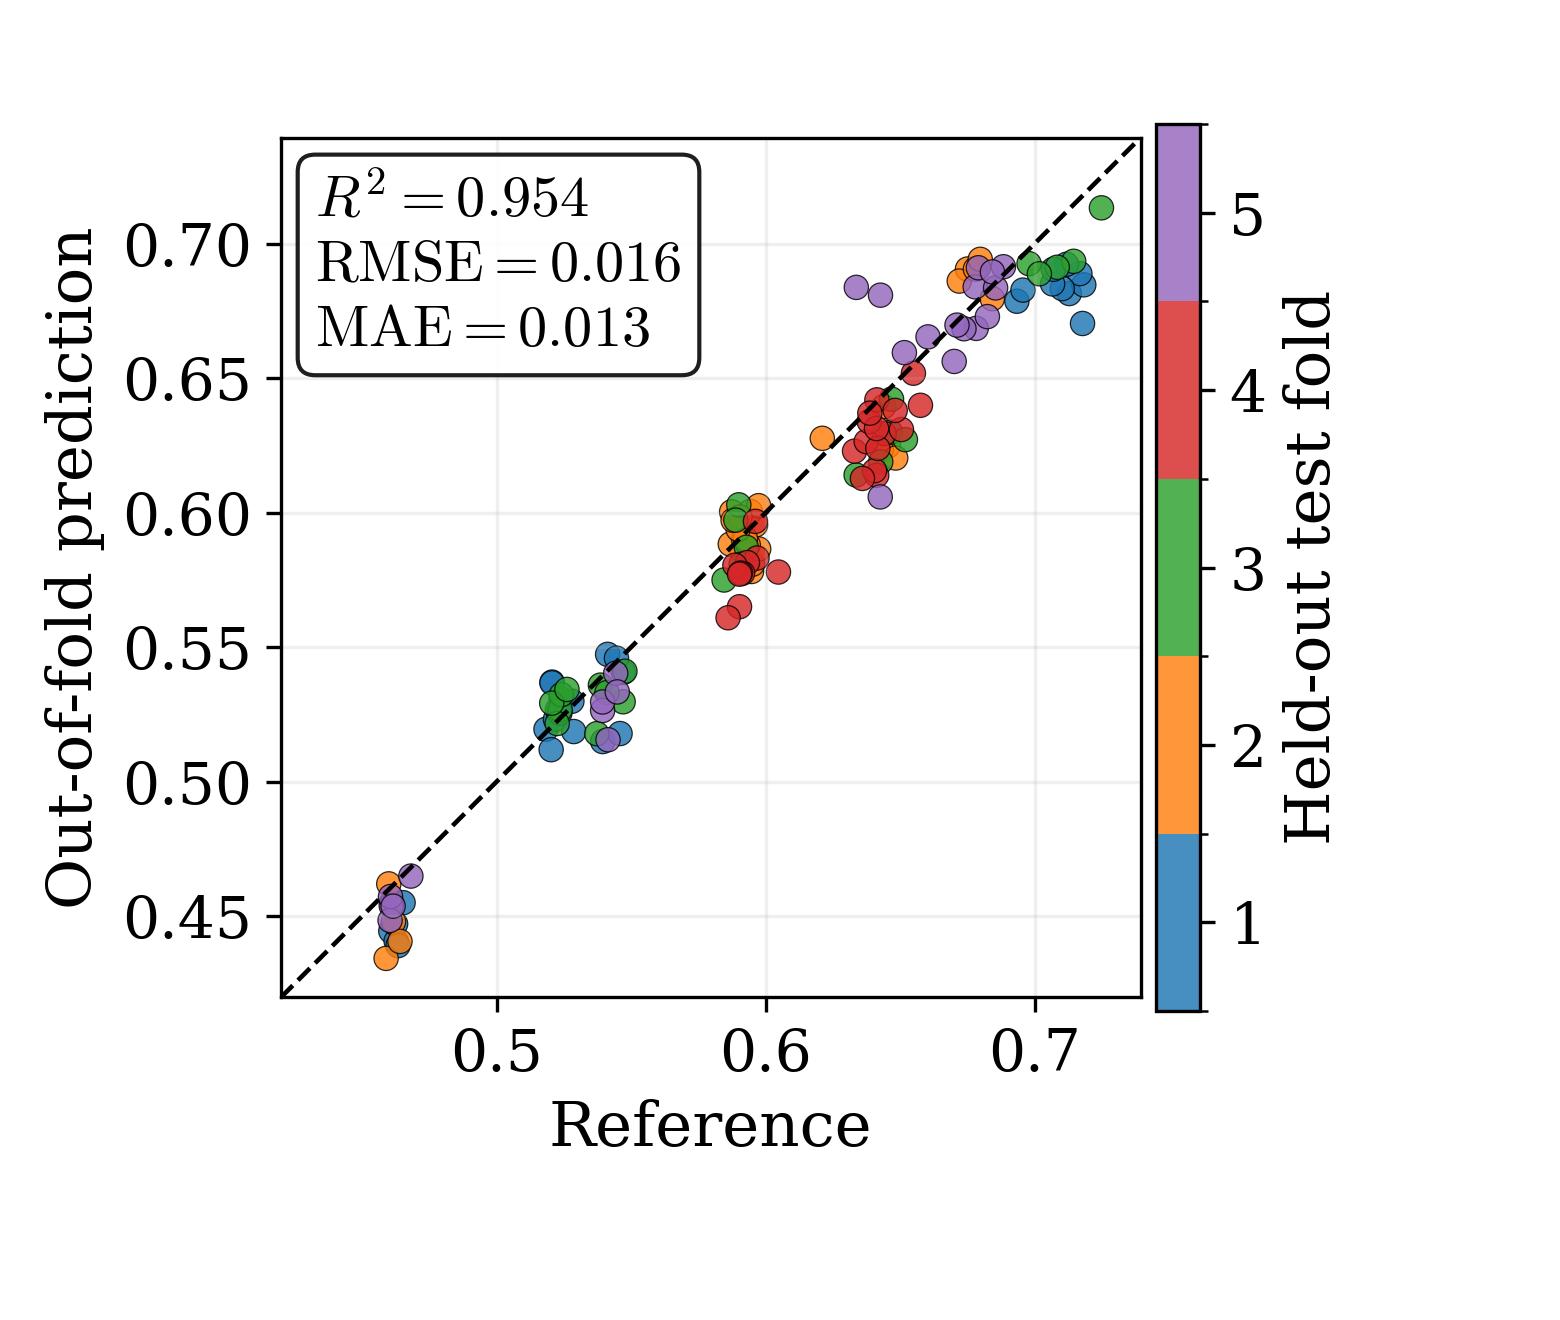
\includegraphics[width=1.\linewidth]{./figures/mean_geometric_exposure_oof_performance.png}%
		}{\fbox{\parbox[c][3.2cm][c]{0.94\linewidth}{\centering
			Out-of-fold parity plot}}}
		\caption{Reference particle-averaged geometric exposure versus its grouped
			out-of-fold GNN prediction. Colours identify the held-out test fold.}
		\label{fig:gnn_oof_performance}
	\end{subfigure}
	\hfill
	\begin{subfigure}[t]{0.49\textwidth}
		\centering
		\IfFileExists{./figures/mean_geometric_exposure_fold_rmse.png}{%
			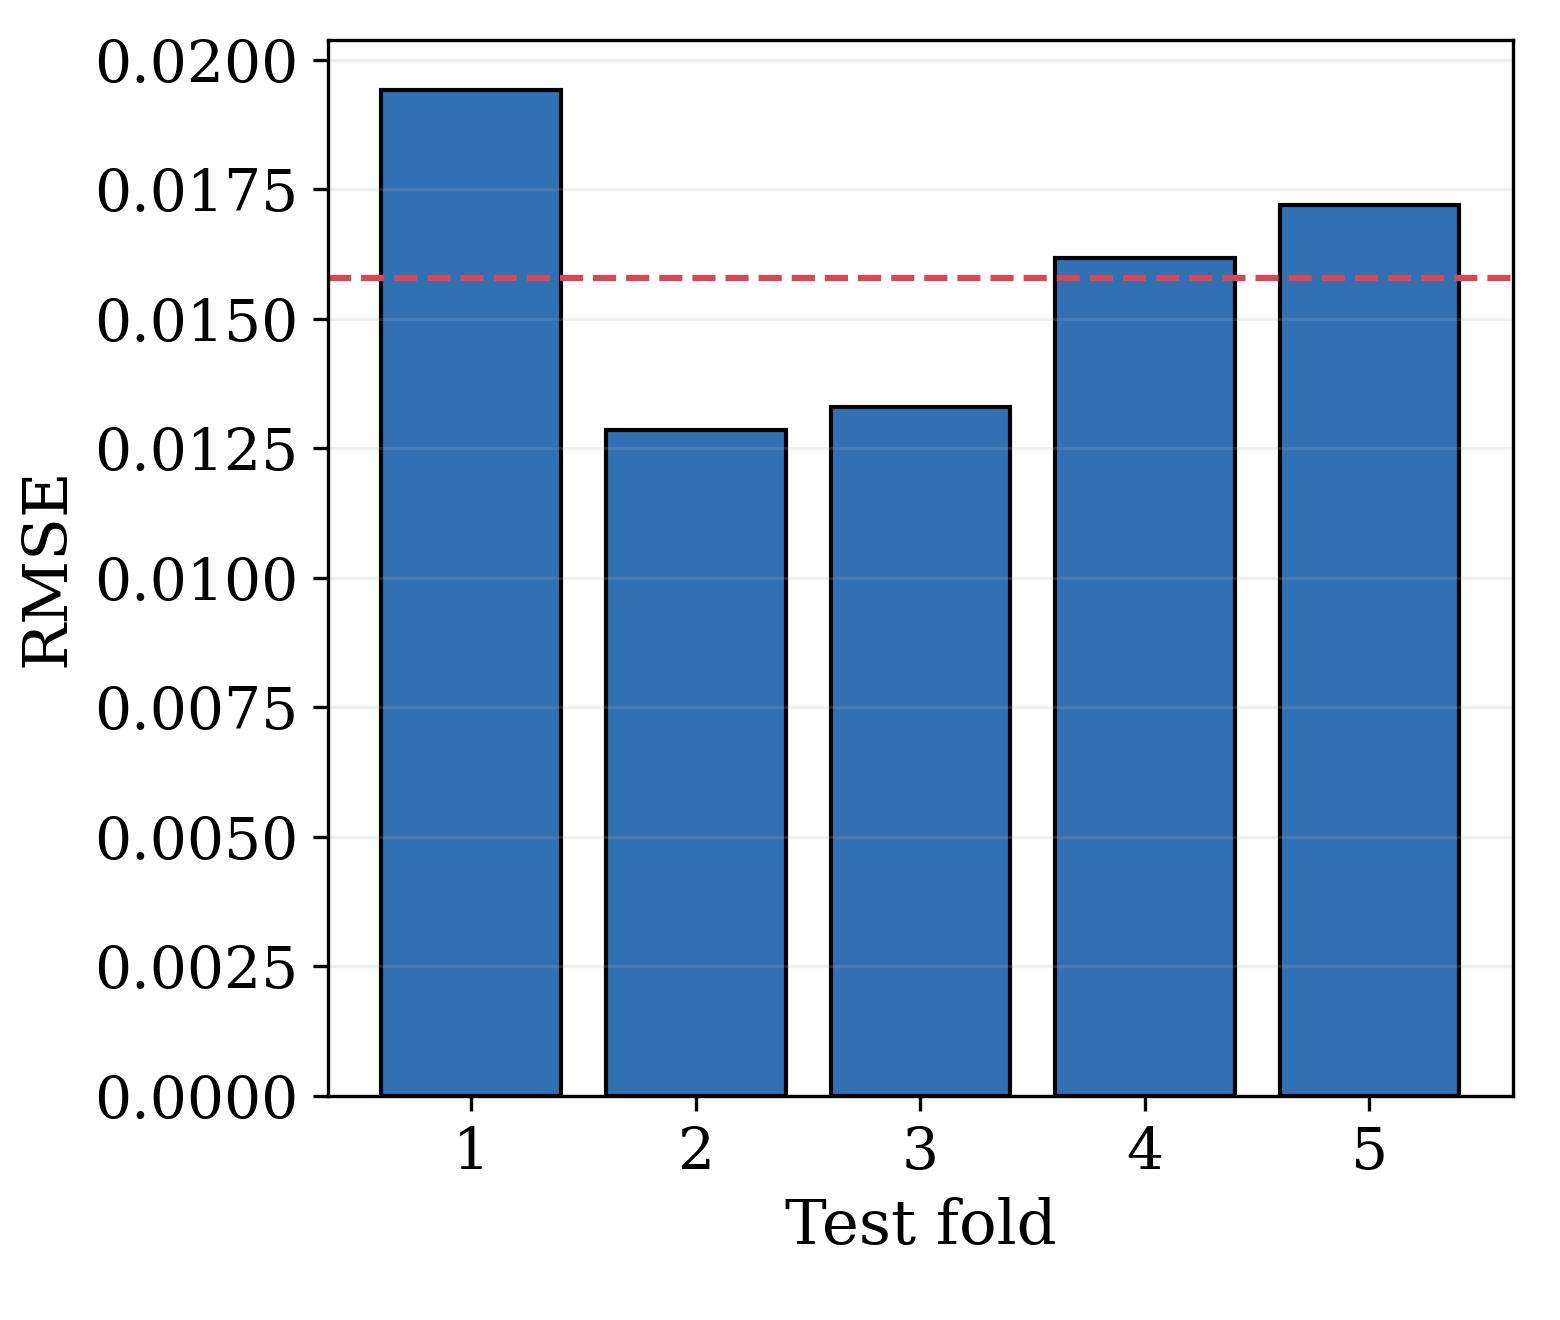
\includegraphics[width=\linewidth]{./figures/mean_geometric_exposure_fold_rmse.png}%
		}{\fbox{\parbox[c][3.2cm][c]{0.94\linewidth}{\centering
			Fold-wise RMSE}}}
		\caption{RMSE in each held-out test fold. The dashed line denotes the mean
			fold RMSE.}
		\label{fig:gnn_fold_rmse}
	\end{subfigure}
	\caption{Prediction of mean geometric exposure with the selected
		one-dimensional GNN under grouped five-fold cross-validation:
		(a) out-of-fold predictions for all 135 agglomerates and
		(b) variation of prediction error among the held-out folds.}
	\label{fig:gnn_cross_validation}
\end{figure}

\subsection{Interpretation of the learned coordinate}

After selecting $n_\lambda=1$, final models were trained on all 135 graphs
using random seeds 7, 17 and 27. Their coordinates were standardized, aligned
in sign and averaged. This all-data coordinate is used only for descriptive
interpretation and not as a leakage-free prediction feature.

Table~\ref{tab:latent_correlations} compares $\lambda_1$ with conventional
descriptors. The strongest monotonic associations were obtained with the
requested fractal dimension ($\rho=-0.800$) and fractal prefactor
($\rho=0.800$). These two effects cannot be separated in the present design
because the three morphology classes pair $D_f$ and $k_f$ one-to-one. Contact
count, particle count and the coordination measures showed moderate negative
associations. In contrast to the former three-target latent coordinate,
$R_g/d_{\mathrm{ref}}$ was essentially uncorrelated with the exposure-specific
coordinate. The arbitrary sign of a one-dimensional latent variable should be
kept in mind: reversing the sign would reverse all reported correlations
without changing the model.

\begin{table}[!tbp]
	\centering
	\caption{Association of the exposure-specific latent coordinate with
		conventional descriptors, ordered by absolute Spearman correlation.}
	\label{tab:latent_correlations}
	\begin{tabular}{lrr}
		\toprule
		Descriptor & Pearson $r$ & Spearman $\rho$ \\
		\midrule
		Requested fractal dimension $D_f$         & -0.789 & -0.800 \\
		Fractal prefactor $k_f$                    &  0.778 &  0.800 \\
		Number of contacts $N_c$                   & -0.579 & -0.596 \\
		Particle count $N$                         & -0.576 & -0.544 \\
		Maximum coordination $z_{\max}$            & -0.555 & -0.541 \\
		Mean coordination $\overline z$            & -0.532 & -0.518 \\
		Contact density $\rho_c$                   &  0.562 &  0.442 \\
		Radius of gyration $R_g/d_{\mathrm{ref}}$  &  0.141 &  0.051 \\
		Primary-particle diameter $d_p$            & -0.003 &  0.000 \\
		\bottomrule
	\end{tabular}
\end{table}

The five realizations in each of the 27 parameter groups had a mean within-group
standard deviation of $0.0586$ in the aligned coordinate, with group values
ranging from $0.0106$ to $0.123$. Thus, stochastic variation within a design
point was small relative to the unit standard deviation of the complete aligned
coordinate.

Grouped-CV regressions were then used to reconstruct $\lambda_1$ from the
available interpretation variables: $d_p$, requested $D_f$, $k_f$, $N$,
$R_g/d_{\mathrm{ref}}$, $N_c$, $\rho_c$, $\overline z$, $z_{\max}$ and the
one-hot-encoded morphology class. The combined random forest reached $R^2=0.991$ and the
combined linear model $R^2=0.988$. The best individual variables were requested
$D_f$ ($R^2=0.557$) and $k_f$ ($R^2=0.536$); no single measured size or contact
descriptor reconstructed the latent coordinate well. These results indicate
that $\lambda_1$ is a compact combination of several morphology attributes,
not a renamed version of particle count or radius of gyration. Because the
all-data GNN generated the interpreted latent values before the reconstruction
cross-validation, this analysis is descriptive rather than a fully nested
independent validation.

\begin{table}[!tbp]
	\centering
	\caption{Grouped-CV reconstruction of the exposure-specific latent
		coordinate from conventional descriptors.}
	\label{tab:latent_reconstruction}
	\begin{tabular}{lr}
		\toprule
		Reconstruction model & $R^2$ \\
		\midrule
		Combined random forest                  & 0.991 \\
		Combined linear model                   & 0.988 \\
		Linear: requested $D_f$                 & 0.557 \\
		Linear: fractal prefactor $k_f$         & 0.536 \\
		Linear: maximum coordination            & 0.262 \\
		Linear: mean coordination               & 0.254 \\
		Linear: contact density                 & 0.250 \\
		Linear: number of contacts              & 0.243 \\
		Linear: particle count                  & 0.238 \\
		Linear: $R_g/d_{\mathrm{ref}}$          & -0.016 \\
		Linear: particle diameter               & -0.066 \\
		\bottomrule
	\end{tabular}
\end{table}

\subsection{Comparison with classical descriptors}

The leakage-free target comparison reused exactly the grouped test folds of the
GNN. The classical models received either one calculated descriptor or the
following six descriptors simultaneously:
\begin{equation}
	N,\quad R_g/d_{\mathrm{ref}},\quad N_c,\quad \rho_c,\quad
	\overline{z},\quad z_{\max}.
\end{equation}
The target $\overline{a}_{\mathrm{geo}}$ was never supplied as an input. A
separate baseline received only the paired requested generation parameters
$D_f$ and $k_f$, without any descriptors calculated from the relaxed
agglomerates.

The pure-graph GNN achieved the highest predictive performance, with
$R^2=0.954$. The linear model combining the six calculated descriptors reached
$R^2=0.922$, whereas the model based only on the requested values of $D_f$ and
$k_f$ reached $R^2=0.604$. Thus, the prescribed morphology class contained
substantial information about geometric exposure but did not reproduce the
realization-, size- and relaxation-dependent variation captured by the
particle graph. Because only the three paired combinations
$(D_f,k_f)=(1.8,1.3)$, $(2.2,1.1)$ and $(2.6,0.8)$ were investigated, the
individual effects of $D_f$ and $k_f$ cannot be separated using the present
dataset.

No individual calculated descriptor approached the performance of the
combined models. The strongest individual result was obtained using a
random-forest model of $R_g/d_{\mathrm{ref}}$, which reached $R^2=0.511$.
Linear maximum coordination reached $R^2=0.296$, whereas the best
particle-count model reached only $R^2=0.160$. The detailed graph therefore
contains predictive information about directional surface obstruction that is
not captured by any individual conventional scalar and is not completely
recovered by their six-variable combination.

\begin{table}[!tbp]
	\centering
	\caption{Grouped out-of-fold prediction of mean geometric exposure. The
		$D_f$--$k_f$ baseline uses only the paired requested generation parameters.
		For each individual calculated descriptor and for the $D_f$--$k_f$
		baseline, the better of the linear and random-forest models is shown.}
	\label{tab:descriptor_baseline}
	\begin{tabular}{lrrr}
		\toprule
		Model or input descriptor & RMSE & MAE & $R^2$ \\
		\midrule
		\textbf{Pure-graph GNN}
		& \textbf{0.0160} & \textbf{0.0128} & \textbf{0.954} \\
		Six descriptors, linear
		& 0.0209 & 0.0183 & 0.922 \\
		Six descriptors, random forest
		& 0.0235 & 0.0168 & 0.902 \\
		Requested $D_f$ and $k_f$, linear
		& 0.0472 & 0.0399 & 0.604 \\
		$R_g/d_{\mathrm{ref}}$, random forest
		& 0.0524 & 0.0383 & 0.511 \\
		Maximum coordination, linear
		& 0.0629 & 0.0516 & 0.296 \\
		Mean coordination, linear
		& 0.0670 & 0.0577 & 0.201 \\
		Number of contacts, linear
		& 0.0685 & 0.0580 & 0.164 \\
		Particle count, linear
		& 0.0687 & 0.0582 & 0.160 \\
		Contact density, linear
		& 0.0701 & 0.0603 & 0.123 \\
		\bottomrule
	\end{tabular}
\end{table}

\section{Conclusions and next steps}
\label{sec:conclusions}

This study establishes an exposure-specific DEM-to-graph-to-GNN workflow for
135 relaxed agglomerates. Geometric exposure is defined by outward-normal
line-of-sight tests over the complete particle surfaces and therefore avoids
classifying accessibility solely through convex-hull membership or contact
depth. The selected one-dimensional GNN predicted this target with grouped
out-of-fold $R^2=0.954$, RMSE $0.0160$ and MAE $0.0128$.

The learned coordinate is task-specific and combines several morphology
attributes. It was most strongly associated with the paired generation
parameters $D_f$ and $k_f$, while particle count and contact-network measures
showed moderate correlations. Conventional descriptors reconstructed the
all-data latent coordinate accurately when combined, but this descriptive
result does not replace leakage-free target evaluation. In the direct target
comparison, the GNN outperformed the best combined classical model
($R^2=0.922$), the paired requested-$D_f$--$k_f$ baseline ($R^2=0.604$), the
best individual descriptor model ($R^2=0.511$), and particle count alone
($R^2=0.160$). Thus, the generation setting explains a substantial part of the
exposure variation, but the detailed relaxed particle graph is needed for the
much higher predictive accuracy obtained here.

The target is nevertheless a geometric proxy. It treats all unobstructed rays
equally and does not account for tortuous diffusion, pore bottlenecks, fluid
motion, oxygen consumption or reaction--transport coupling. The next stage
should examine ray-number convergence and probe-radius sensitivity, expand the
morphology ensemble, and compare $\overline a_{\mathrm{geo}}$ with oxygen
uptake, response time and oxygen-limited particle fractions obtained from
resolved transport calculations. That comparison will establish whether the
present exposure coordinate is physically useful or must be supplemented by
transport-aware graph information.

\printbibliography

%\begin{thebibliography}{99}
%
%\bibitem{Filippov2000}
%A.~V. Filippov, M.~Zurita, and D.~E. Rosner,
%``Fractal-like aggregates: relation between morphology and physical
%properties,''
%\emph{Journal of Colloid and Interface Science}, vol.~229,
%pp.~261--273, 2000.
%\href{https://doi.org/10.1006/jcis.2000.7027}{doi:10.1006/jcis.2000.7027}.
%
%\bibitem{Skorupski2014}
%K.~Skorupski, J.~Mroczka, T.~Wriedt, and N.~Riefler,
%``A fast and accurate implementation of tunable algorithms used for generation
%of fractal-like aggregate models,''
%\emph{Physica A}, vol.~404, pp.~106--117, 2014.
%\href{https://doi.org/10.1016/j.physa.2014.02.072}{doi:10.1016/j.physa.2014.02.072}.
%
%\bibitem{Ehrl2009}
%L.~Ehrl, M.~Soos, and M.~Lattuada,
%``Generation and geometrical analysis of dense clusters with variable fractal
%dimension,''
%\emph{Journal of Physical Chemistry B}, vol.~113,
%pp.~10587--10599, 2009.
%\href{https://doi.org/10.1021/jp903557m}{doi:10.1021/jp903557m}.
%
%\bibitem{LevinAngert2015}
%P.~A. Levin and E.~R. Angert,
%``Small but mighty: cell size and bacteria,''
%\emph{Cold Spring Harbor Perspectives in Biology}, vol.~7, a019216, 2015.
%\href{https://doi.org/10.1101/cshperspect.a019216}{doi:10.1101/cshperspect.a019216}.
%
%\bibitem{MartinezSalas1981}
%E.~Mart\'inez-Salas, J.~A. Mart\'in, and M.~Vicente,
%``Relationship of \textit{Escherichia coli} density to growth rate and cell
%age,''
%\emph{Journal of Bacteriology}, vol.~147, pp.~97--100, 1981.
%\href{https://doi.org/10.1128/jb.147.1.97-100.1981}{doi:10.1128/jb.147.1.97-100.1981}.
%
%\bibitem{Woldringh1981}
%C.~L. Woldringh, J.~S. Binnerts, and A.~Mans,
%``Variation in \textit{Escherichia coli} buoyant density measured in Percoll
%gradients,''
%\emph{Journal of Bacteriology}, vol.~148, pp.~58--63, 1981.
%\href{https://doi.org/10.1128/jb.148.1.58-63.1981}{doi:10.1128/jb.148.1.58-63.1981}.
%
%\bibitem{Deng2011}
%Y.~Deng, M.~Sun, and J.~W. Shaevitz,
%``Direct measurement of cell wall stress stiffening and turgor pressure in
%live bacterial cells,''
%\emph{Physical Review Letters}, vol.~107, 158101, 2011.
%\href{https://doi.org/10.1103/PhysRevLett.107.158101}{doi:10.1103/PhysRevLett.107.158101}.
%
%\bibitem{Lee2024}
%J.~Lee, K.~Jha, C.~E. Harper, W.~Zhang, and M.~Ramsukh,
%``Determining the Young's modulus of the bacterial cell envelope,''
%\emph{ACS Biomaterials Science \& Engineering}, vol.~10,
%pp.~2956--2966, 2024.
%\href{https://doi.org/10.1021/acsbiomaterials.4c00105}{doi:10.1021/acsbiomaterials.4c00105}.
%
%\bibitem{Hamaker1937}
%H.~C. Hamaker,
%``The London--van der Waals attraction between spherical particles,''
%\emph{Physica}, vol.~4, pp.~1058--1072, 1937.
%\href{https://doi.org/10.1016/S0031-8914(37)80203-7}{doi:10.1016/S0031-8914(37)80203-7}.
%
%\bibitem{Israelachvili2011}
%J.~N. Israelachvili,
%\emph{Intermolecular and Surface Forces}, 3rd~ed.
%Academic Press, 2011.
%\bibitem{Bushell2002}
%G.~C. Bushell, Y.~D. Yan, D.~Woodfield, J.~Raper, and R.~Amal,
%``On techniques for the measurement of the mass fractal dimension of
%aggregates,''
%\emph{Advances in Colloid and Interface Science}, vol.~95, no.~1,
%pp.~1--50, 2002.
%\href{https://doi.org/10.1016/S0001-8686(00)00078-6}
%{doi:10.1016/S0001-8686(00)00078-6}.
%
%\bibitem{Sorensen2001}
%C.~M. Sorensen,
%``Light scattering by fractal aggregates: A review,''
%\emph{Aerosol Science and Technology}, vol.~35, no.~2,
%pp.~648--687, 2001.
%\href{https://doi.org/10.1080/02786820117868}
%{doi:10.1080/02786820117868}.
%
%\bibitem{Theiler1990}
%J.~Theiler,
%``Estimating fractal dimension,''
%\emph{Journal of the Optical Society of America A}, vol.~7, no.~6,
%pp.~1055--1073, 1990.
%\href{https://doi.org/10.1364/JOSAA.7.001055}
%{doi:10.1364/JOSAA.7.001055}.
%
%\bibitem{ForoutanPour1999}
%K.~Foroutan-pour, P.~Dutilleul, and D.~L. Smith,
%``Advances in the implementation of the box-counting method of fractal
%dimension estimation,''
%\emph{Applied Mathematics and Computation}, vol.~105, nos.~2--3,
%pp.~195--210, 1999.
%\href{https://doi.org/10.1016/S0096-3003(98)10096-6}
%{doi:10.1016/S0096-3003(98)10096-6}.
%
%\bibitem{Liebovitch1989}
%L.~S. Liebovitch and T.~Toth,
%``A fast algorithm to determine fractal dimensions by box counting,''
%\emph{Physics Letters A}, vol.~141, nos.~8--9,
%pp.~386--390, 1989.
%\href{https://doi.org/10.1016/0375-9601(89)90854-2}
%{doi:10.1016/0375-9601(89)90854-2}.
%
%\end{thebibliography}

\end{document}
